
\section{Evaluating Topic Models}

\begin{frame}
  \vspace{-2cm}
  \begin{columns}
    \column{.45\linewidth}
    \begin{center}
      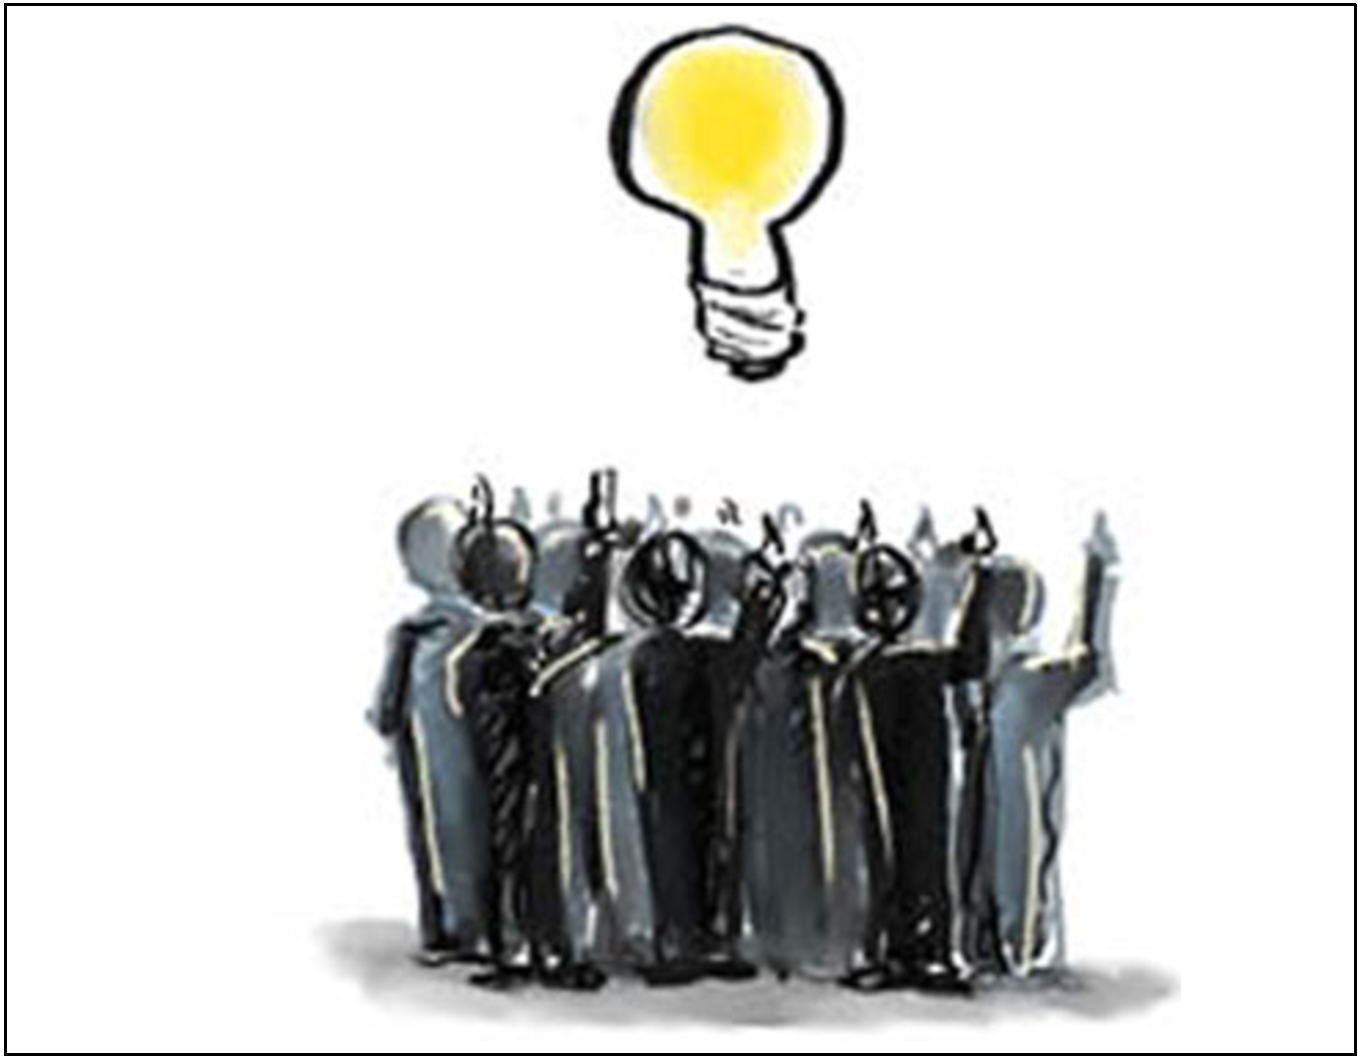
\includegraphics[width=\linewidth]{cognitive/crowdsourcing_on}
      \end{center}
    \column{.45\linewidth}
    \begin{center}
      
\includegraphics[width=\linewidth]{cognitive/user_off}
      \end{center}

  \end{columns}

  \begin{columns}
    \column{.45\linewidth}
    \begin{center}
      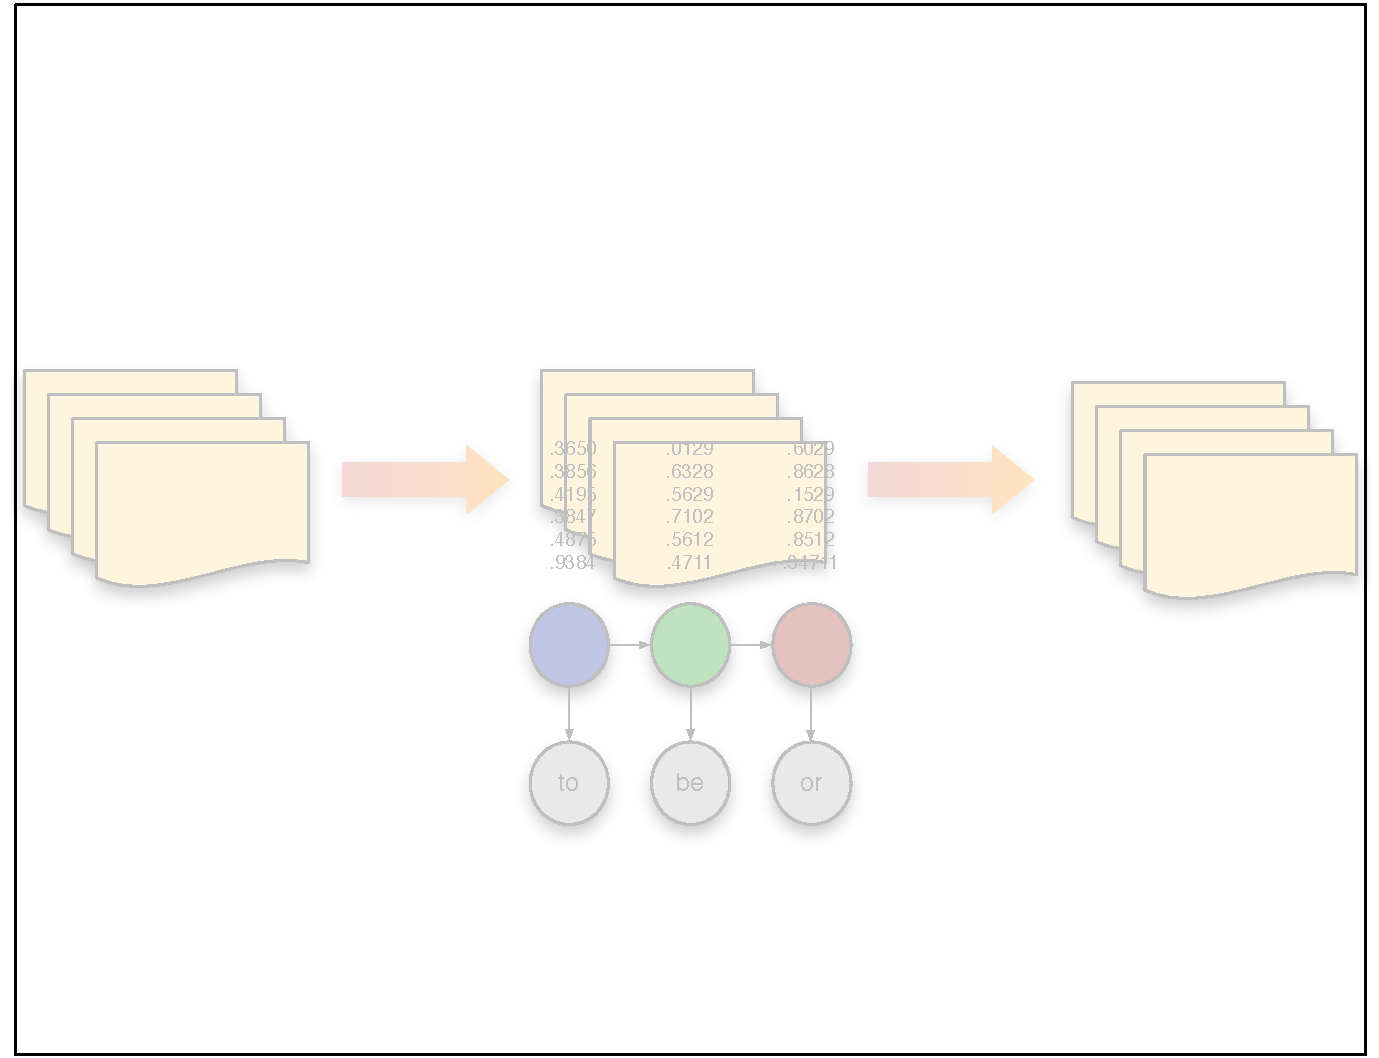
\includegraphics[width=\linewidth]{cognitive/algorithms_off}
      \end{center}
    \column{.45\linewidth}
    \begin{center}
      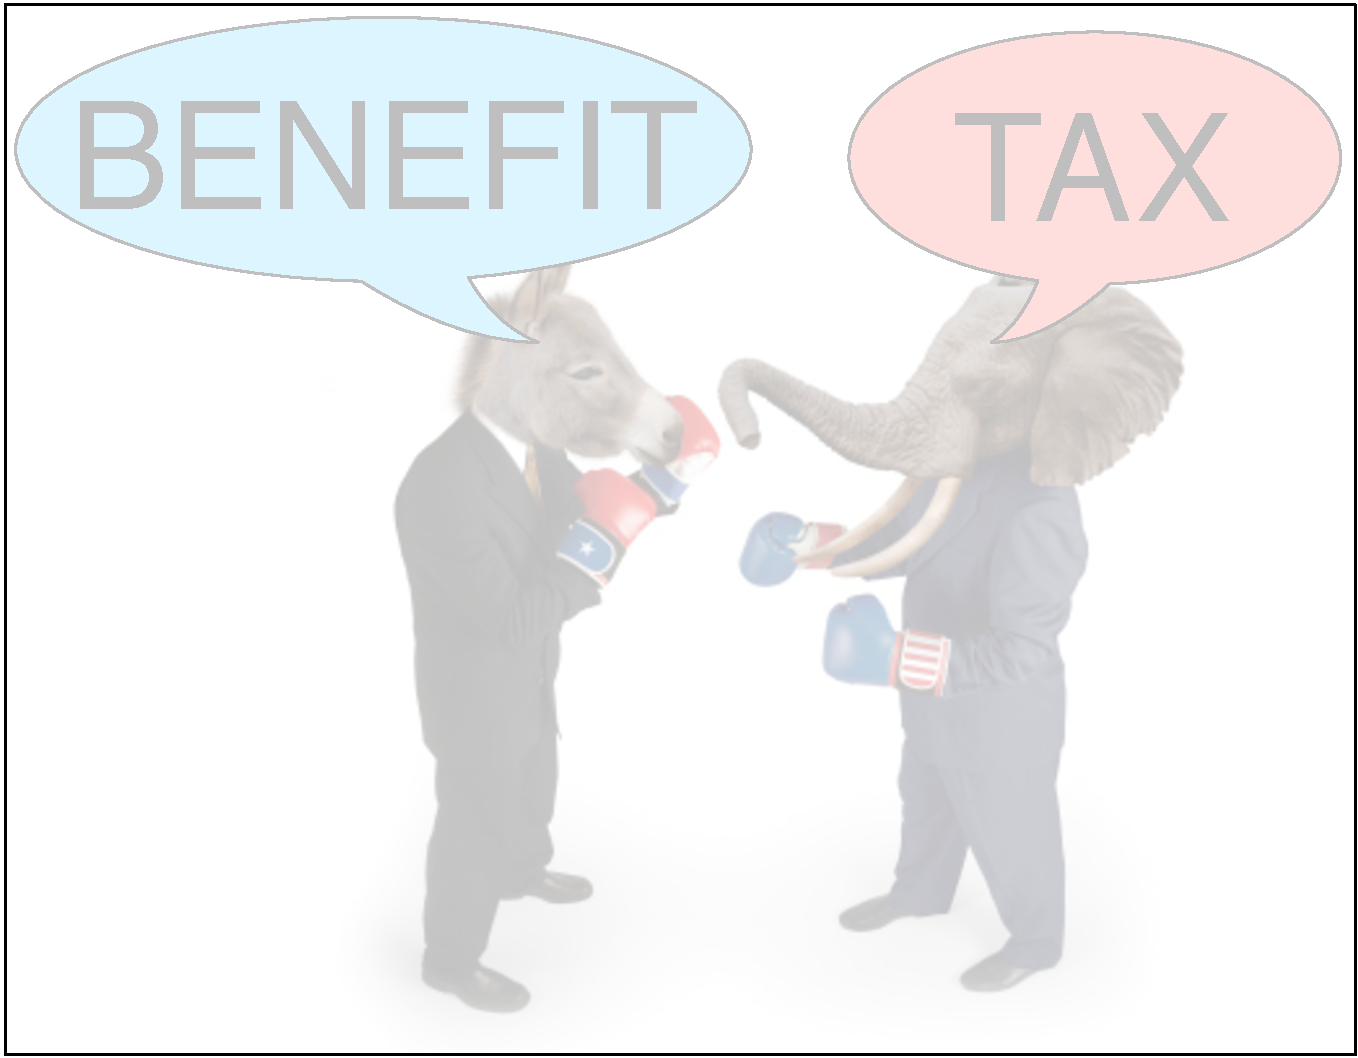
\includegraphics[width=\linewidth]{cognitive/framing_off}
      \end{center}
  \end{columns}

\only<2->{
\vspace{-3cm}
\begin{block}{Reading Tea Leaves}
        How we used to evaluate topic models was wrong; but there is a better
        way using crowdsourcing
\end{block}
}

\end{frame}

\begin{frame}{Evaluating Topic Models}

\begin{columns}

\column{.6\linewidth}
\begin{block}{ Reading Tea Leaves: How Humans Interpret Topic Models}
Jonathan Chang, Jordan Boyd-Graber, Chong Wang, Sean Gerrish, and David
M. Blei. Reading Tea Leaves: How Humans Interpret Topic Models. Neural
Information Processing Systems, 2009.
\end{block}

{\bf Jonathan and I shared a NIPS 2009 Best Student Paper HM}

\column{.3\linewidth}
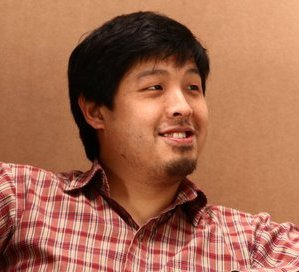
\includegraphics[width=.8\linewidth]{general_figures/jonathan}

\end{columns}

\end{frame}



\frame{
\frametitle{Evaluation}
\begin{center}
%\only<1>{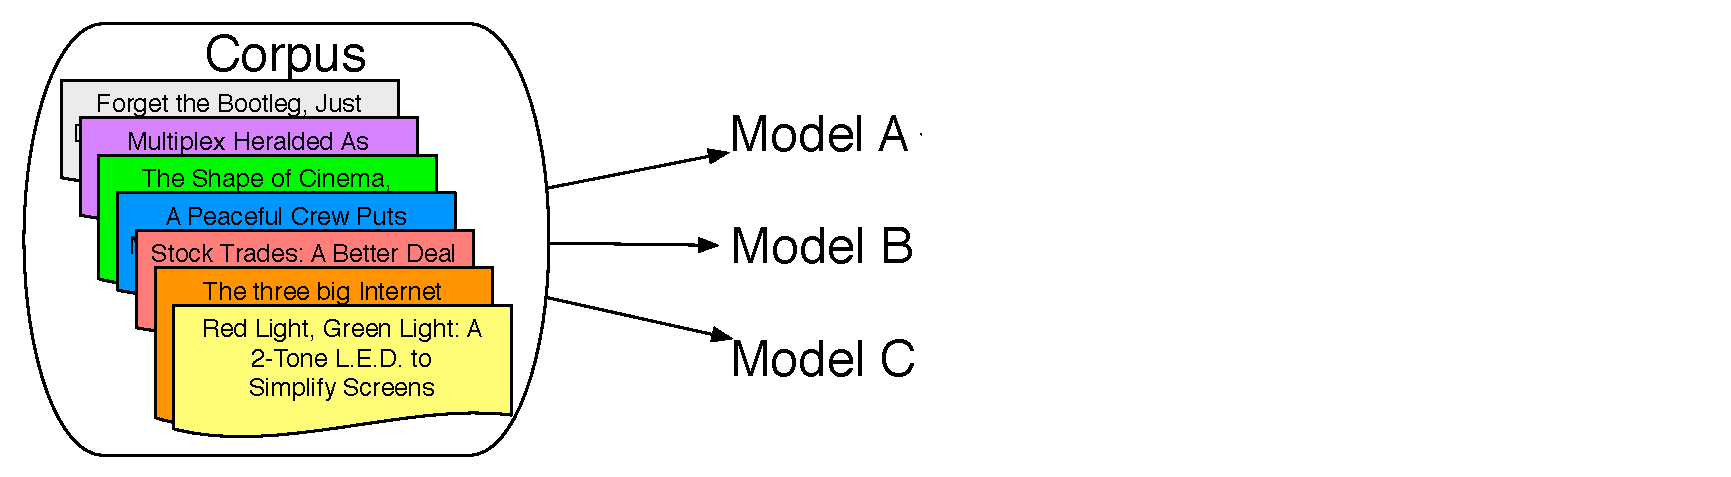
\includegraphics[width=0.9\linewidth]{reading_tea_leaves/figures/heldout_1} }
\only<1>{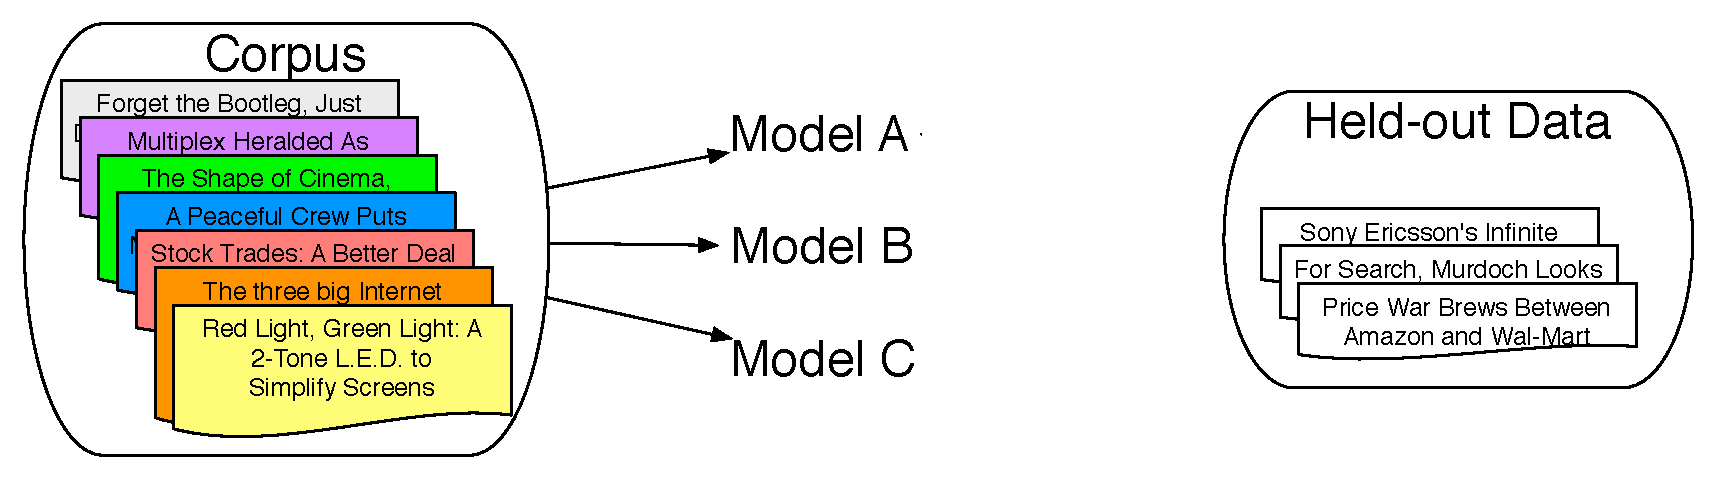
\includegraphics[width=\linewidth]{reading_tea_leaves/figures/heldout_2} }
%\only<3>{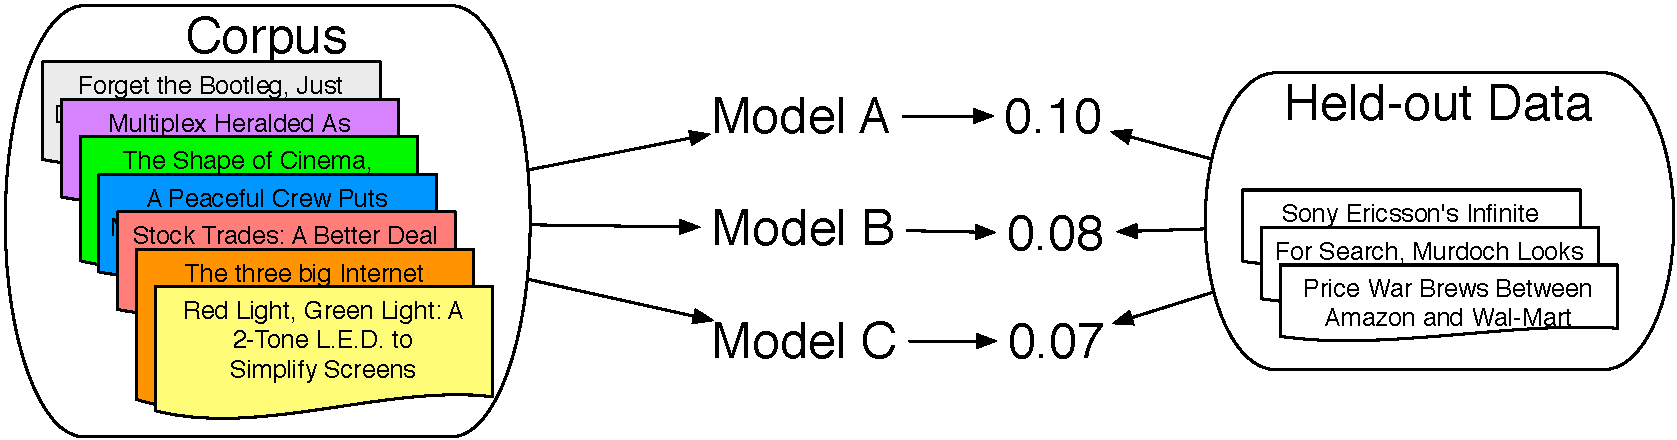
\includegraphics[width=\linewidth]{reading_tea_leaves/figures/heldout_3} }
\only<2>{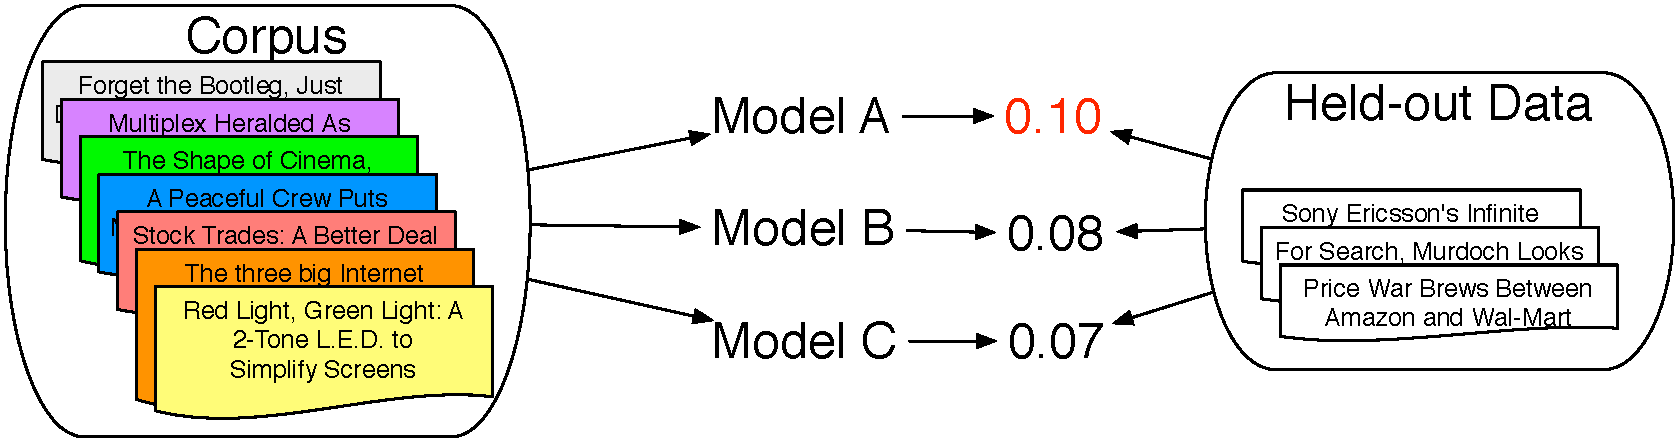
\includegraphics[width=\linewidth]{reading_tea_leaves/figures/heldout_4}  \\
	\large Measures predictive power (likelihood / perplexity)}
\end{center}
}


\frame{
        \frametitle{Interruption}

  \begin{columns}
  \column{.6\linewidth}
  \begin{block}{Do you have any real results?}
  \centering
     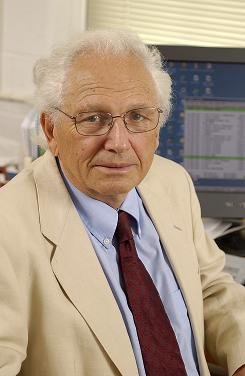
\includegraphics[width=0.5\linewidth]{reading_tea_leaves/jelinek} \\
     Fred Jelinek, inventor of perplexity~\cite{jelinek-76}
  \end{block}

  \column{.4\linewidth}

  \begin{itemize}
    \item Computational linguists and machine learning researchers like {\bf numbers}
    \item Likelihood and perplexity are convenient numbers
    \pause
    \item What do we {\bf actually} care about in topic models?
  \end{itemize}

  \end{columns}
}

\frame{
\frametitle{Qualitative Evaluation of the Latent Space}

\begin{center}
\only<1>{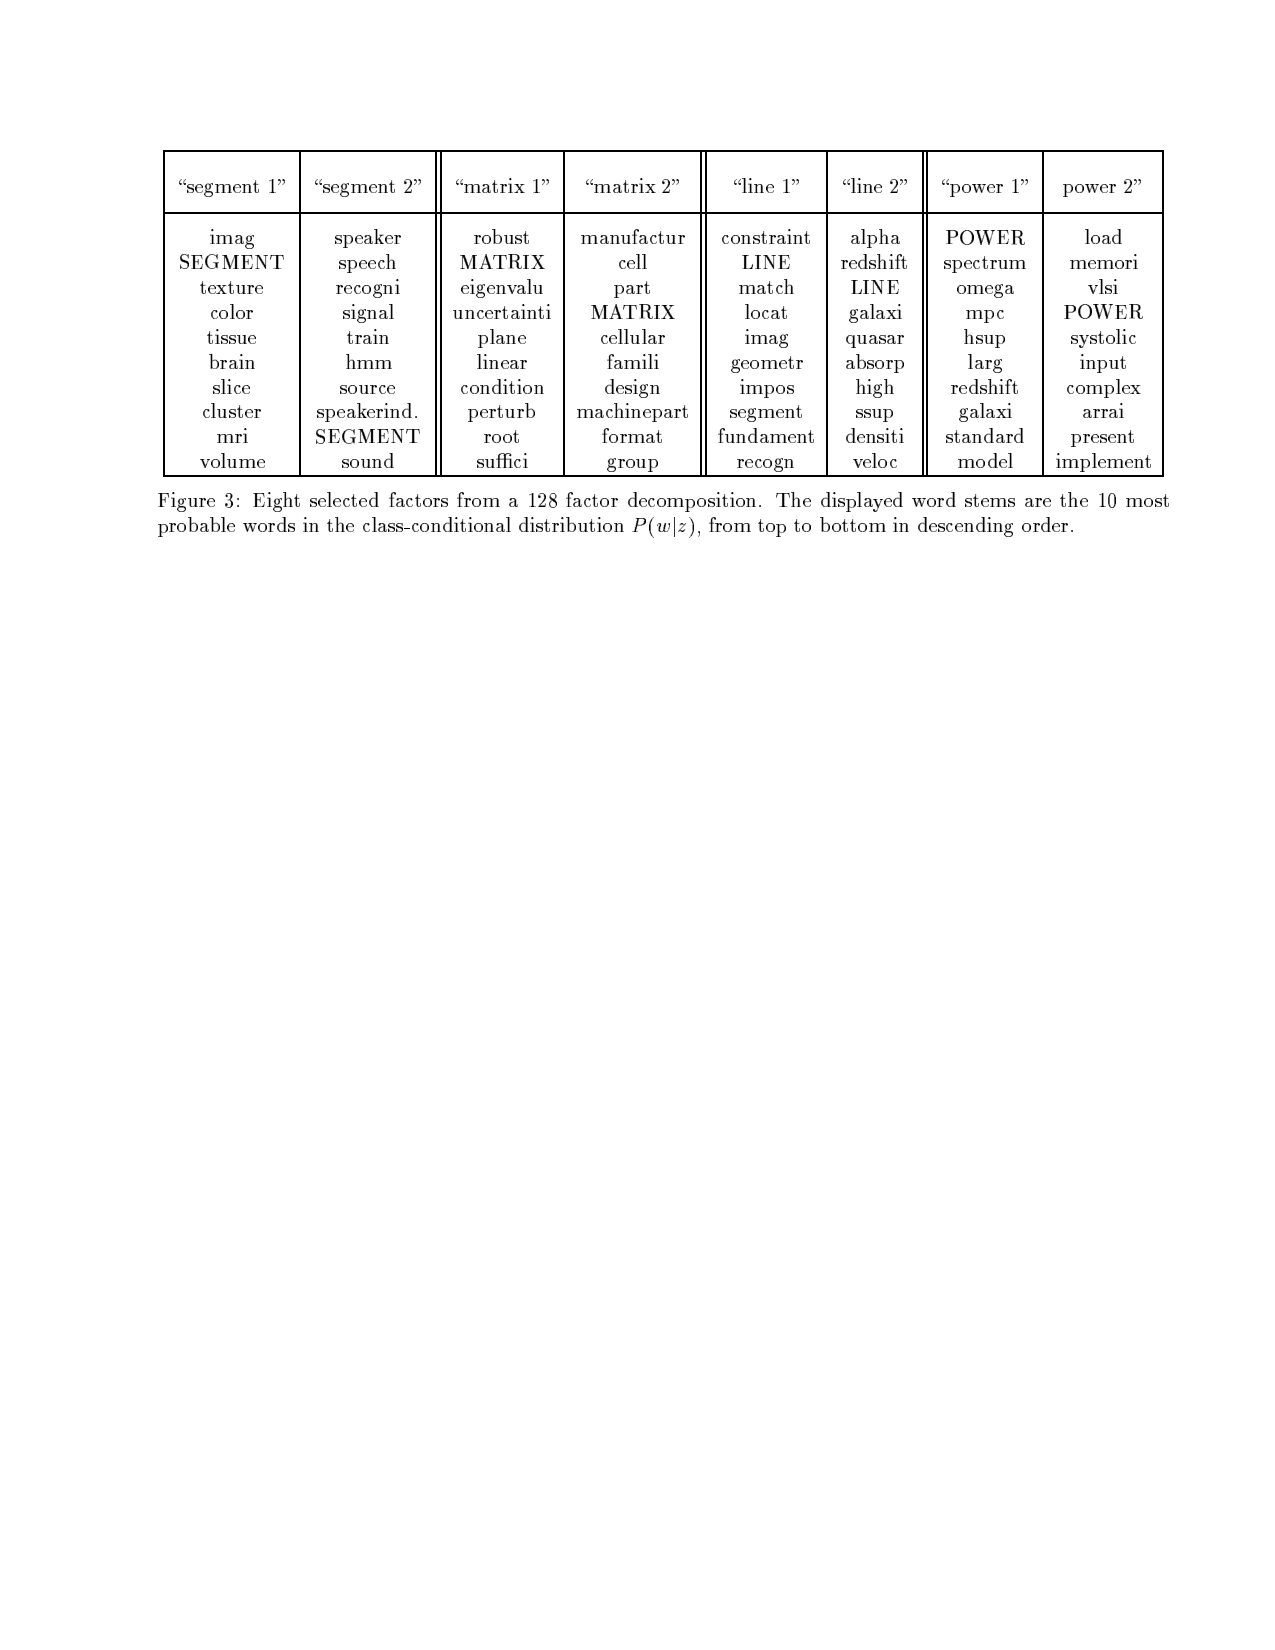
\includegraphics[width=0.9\linewidth]{reading_tea_leaves/topics_from_papers/1} \\ \cite{hofmann-99} }
\only<2>{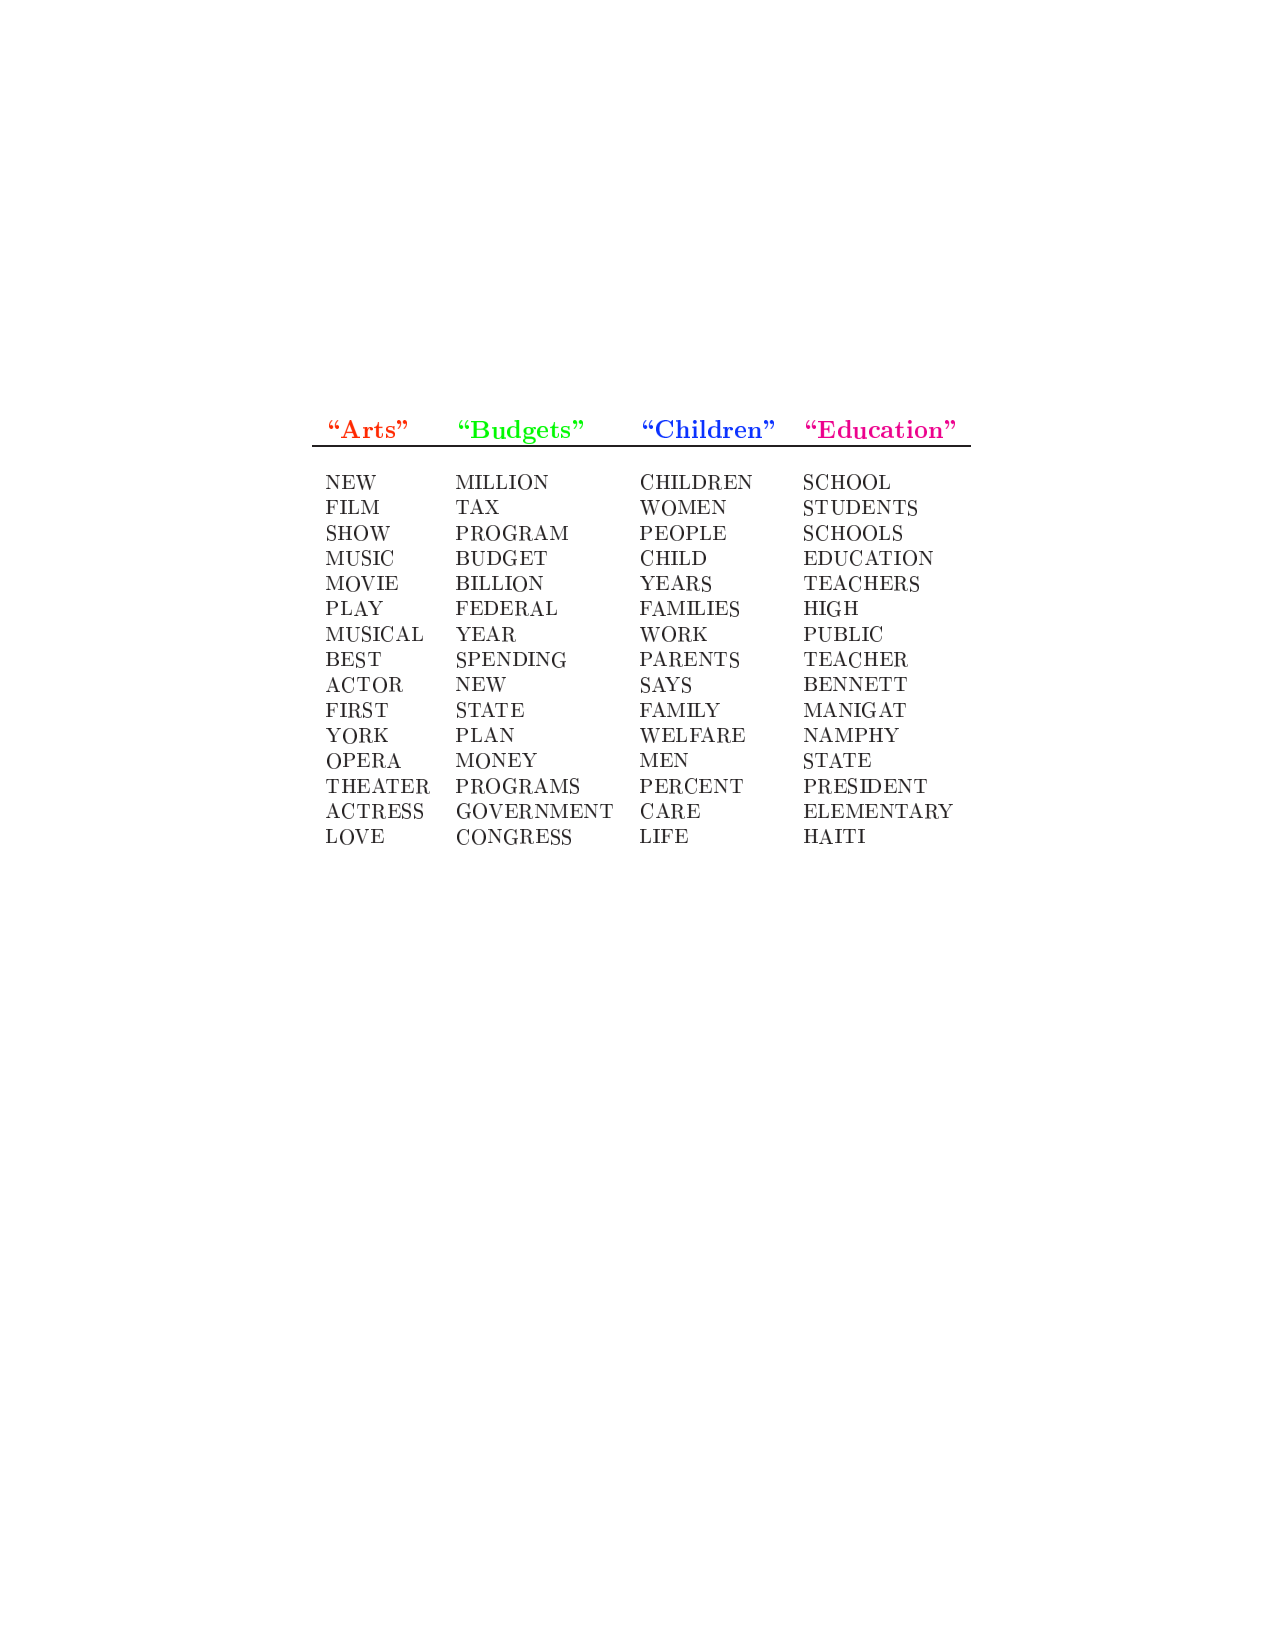
\includegraphics[width=0.7\linewidth]{reading_tea_leaves/topics_from_papers/2} \\ \cite{blei-03} }
\only<3>{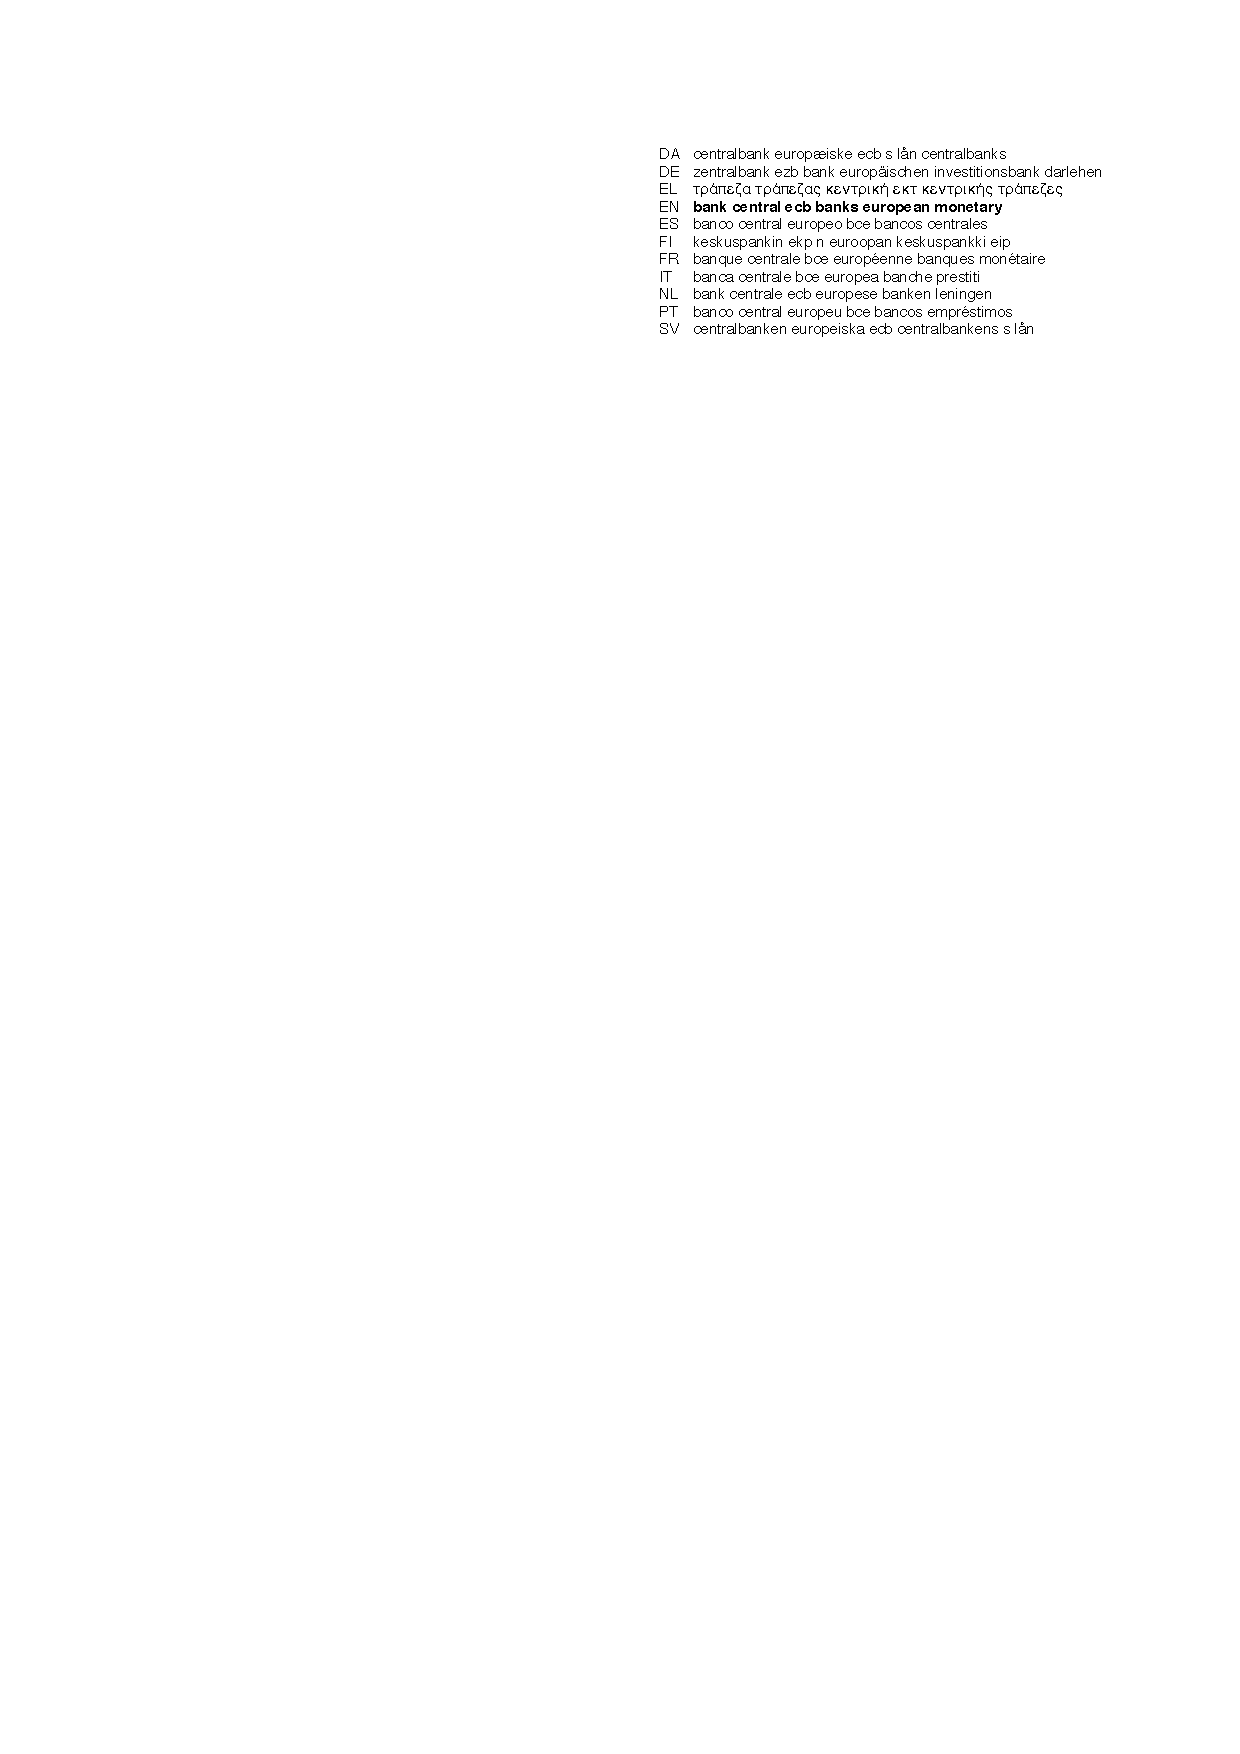
\includegraphics[width=0.7\linewidth]{reading_tea_leaves/topics_from_papers/3} \\ \cite{mimno-09} }
\only<4>{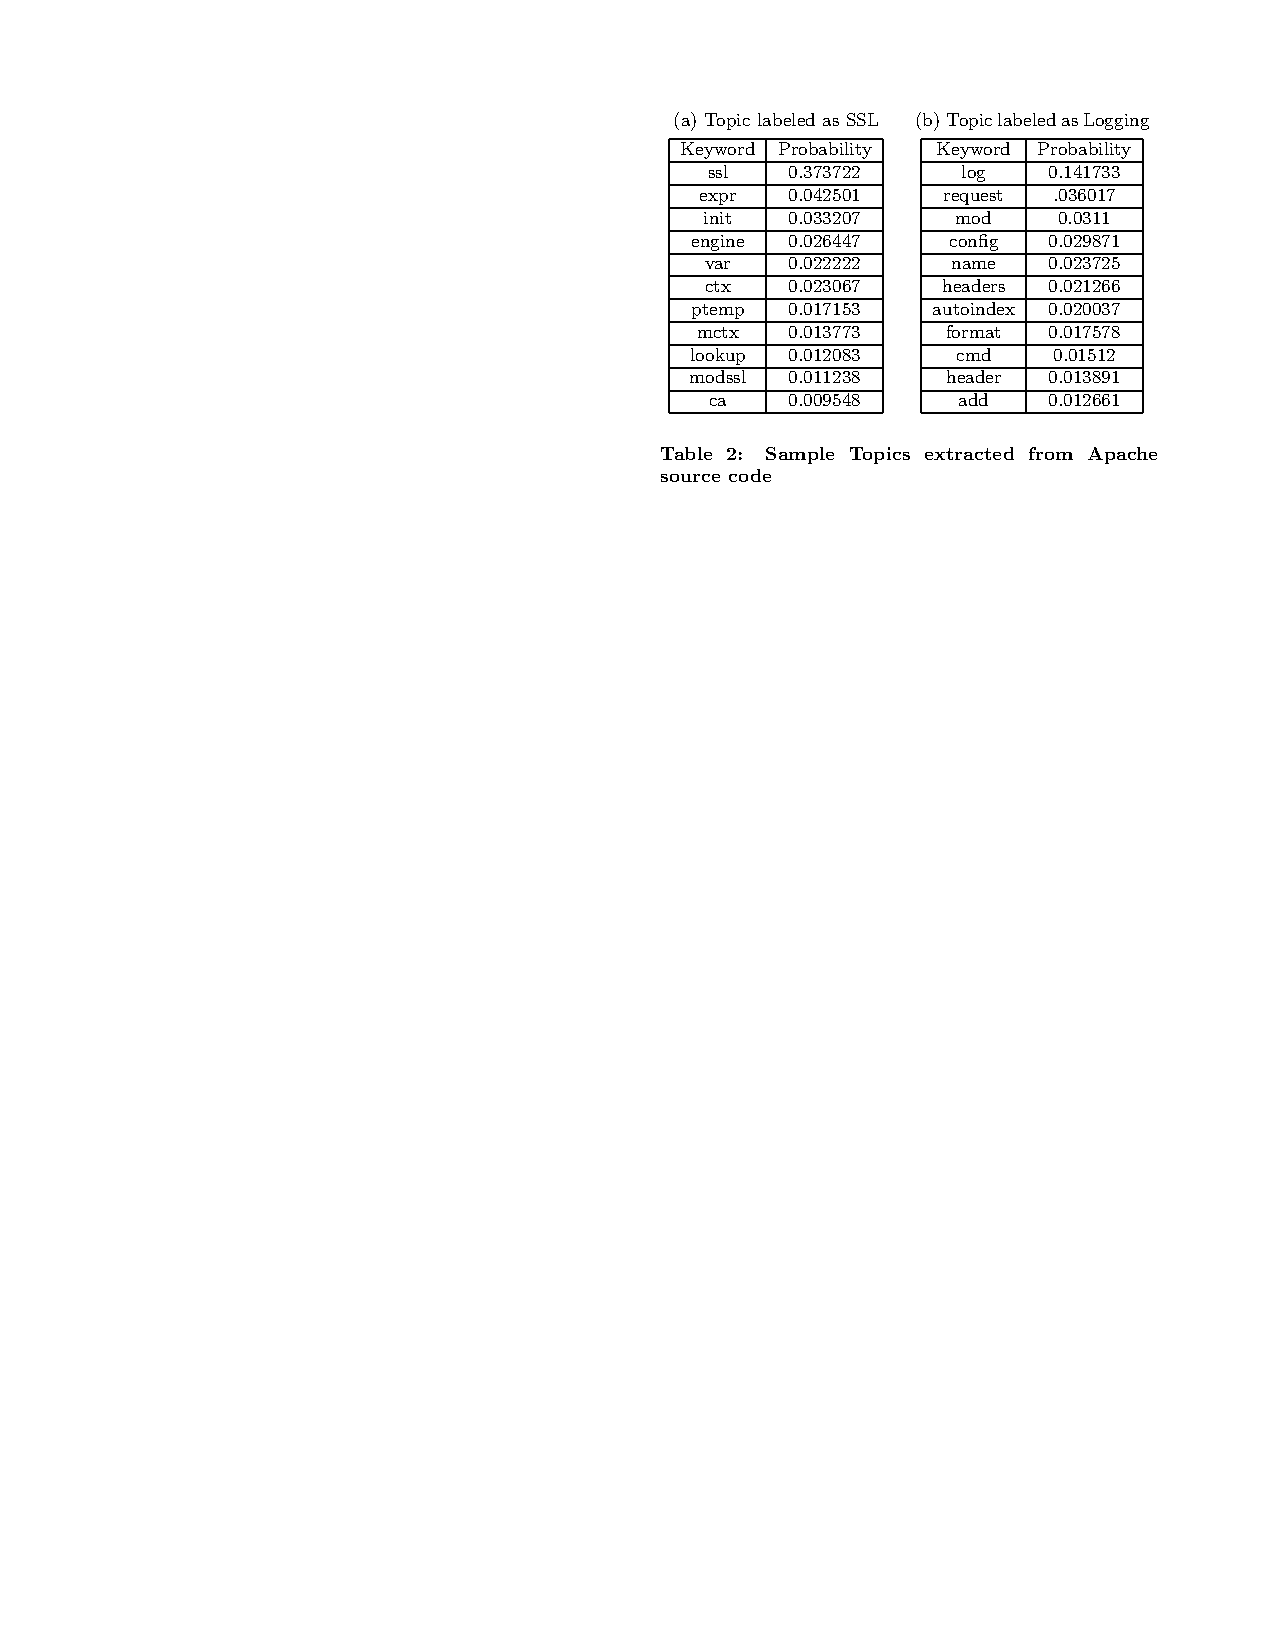
\includegraphics[width=0.7\linewidth]{reading_tea_leaves/topics_from_papers/4} \\ \cite{maskeri-08} }

\only<5->{
\begin{block}{Interpretability}
        When a user looks at a topic, does it make sense?
\end{block}
\pause
  \begin{itemize}
   \item Interpretability is a human judgment
    \item We will ask people directly
    \item Experiment Goals
      \begin{itemize}
        \item Quick
        \item Fun
        \item Consistent
      \end{itemize}
      \pause
      \item We turn to Amazon Mechanical Turk
        \iflong
       \item Two tasks: Word Intrusion and Topic Intrusion
         \else
         \item Primary task: Word Intrusion
         \fi

  \end{itemize}
}
\end{center}
}

\frame{
\frametitle{Data from the Cloud}
\begin{columns}[c]


\column{0.45\linewidth}

\begin{block}{Then}
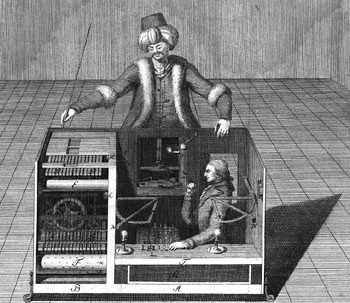
\includegraphics[width=0.95\linewidth]{evocation/figures/mechanical_turk_old}
\end{block}


\column{0.45\linewidth}

\begin{block}{Now}
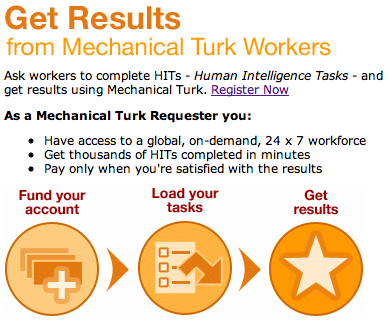
\includegraphics[width=0.95\linewidth]{evocation/figures/mechanical_turk_new}
\end{block}

\end{columns}
}

\frame{
  \frametitle{Word Intrusion}

  \begin{enumerate}
    \item Take the highest probability words from a topic

      \begin{block}{Original Topic}
        dog, cat, horse, pig, cow
      \end{block}
\pause
    \item Take a high-probability word from another topic and add it
      \begin{block}{Topic with Intruder}
        dog, cat, \alert<2->{apple}, horse, pig, cow
      \end{block}
\pause
     \item We ask users to find the word that doesn't belong
  \end{enumerate}
\begin{block}{Hypothesis}
If the topics are interpretable, users will consistently choose true intruder
\end{block}
}

\frame{
  \frametitle{Word Intrusion}

\begin{center}
\only<1>{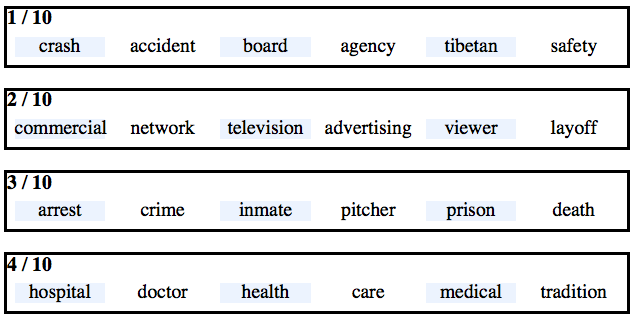
\includegraphics[width=\linewidth]{reading_tea_leaves/tasks/word1}  }
\only<2>{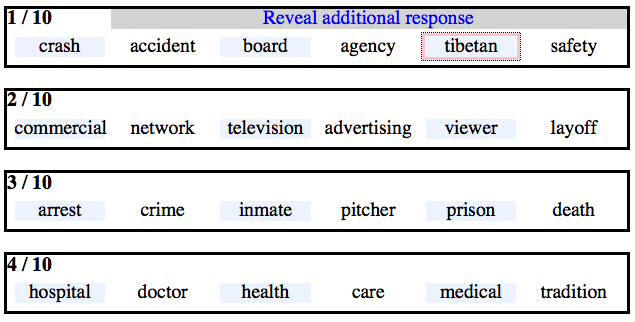
\includegraphics[width=\linewidth]{reading_tea_leaves/tasks/word2}  }
\pause
  \begin{itemize}
    \item Order of words was shuffled
    \item Which intruder was selected varied
    \item Model precision: percentage of users who clicked on intruder
  \end{itemize}

\end{center}
}


\frame{
\frametitle{Word Intrusion: Which Topics are Interpretable?}
  \begin{block}{New York Times, 50 Topics}
    \begin{center}
      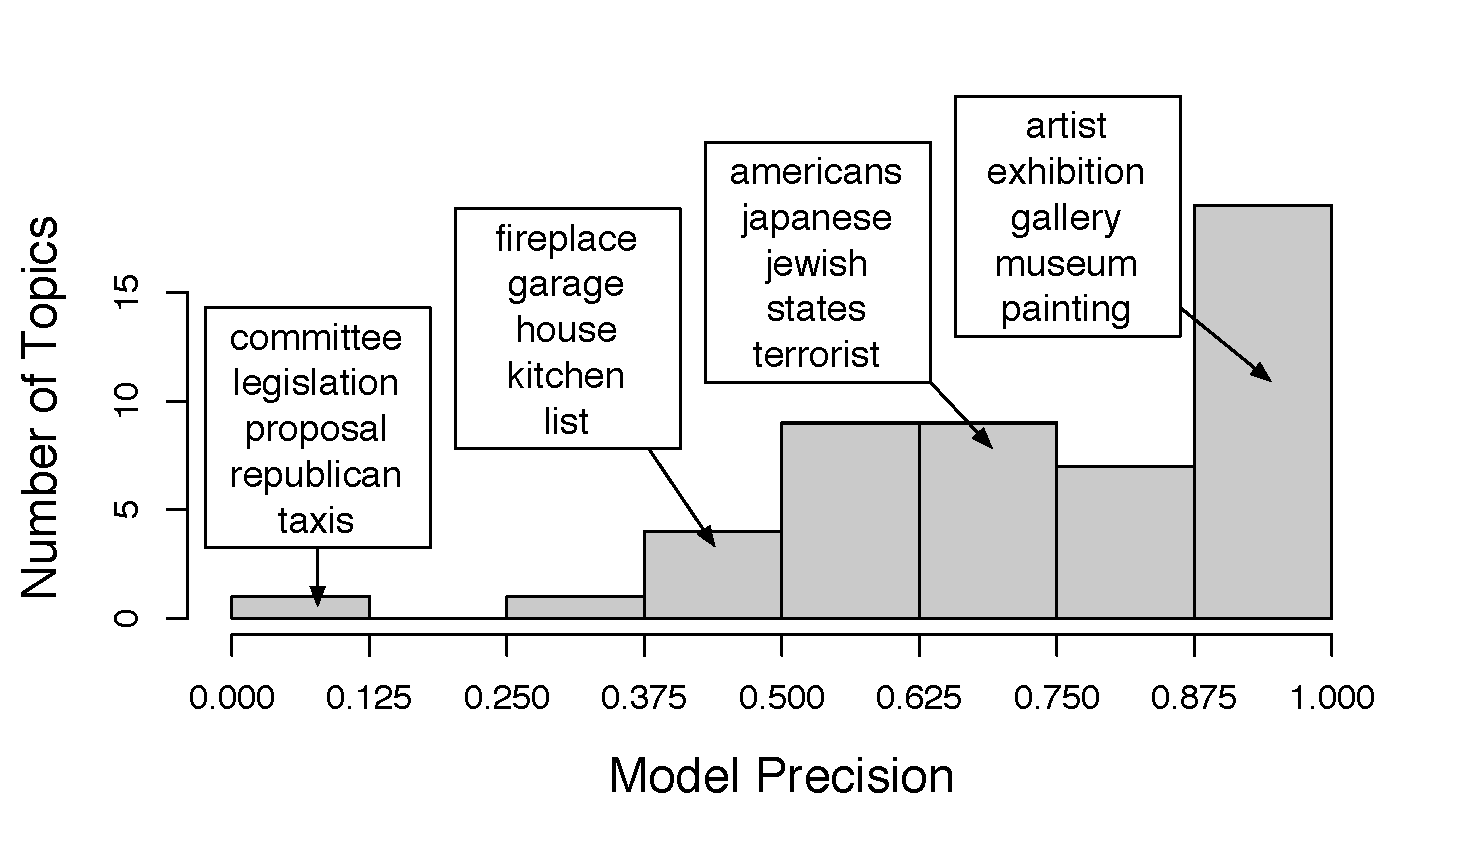
\includegraphics[width=0.8\linewidth]{reading_tea_leaves/figures/topic_precision}
    \end{center}
  \end{block}
  \begin{center}
    Model Precision: percentage of correct intruders found
  \end{center}
}

\frame{

\frametitle{Interpretability and Likelihood}

\begin{center}
\only<1>{Model Precision on New York Times}
\end{center}

\begin{columns}
\column{.84\linewidth}
\begin{flushright}
  \only<1>{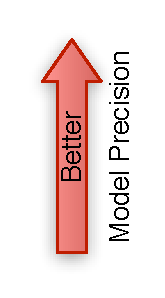
\includegraphics[scale=\graphscale]{reading_tea_leaves/tasks/mp}}
  \only<1>{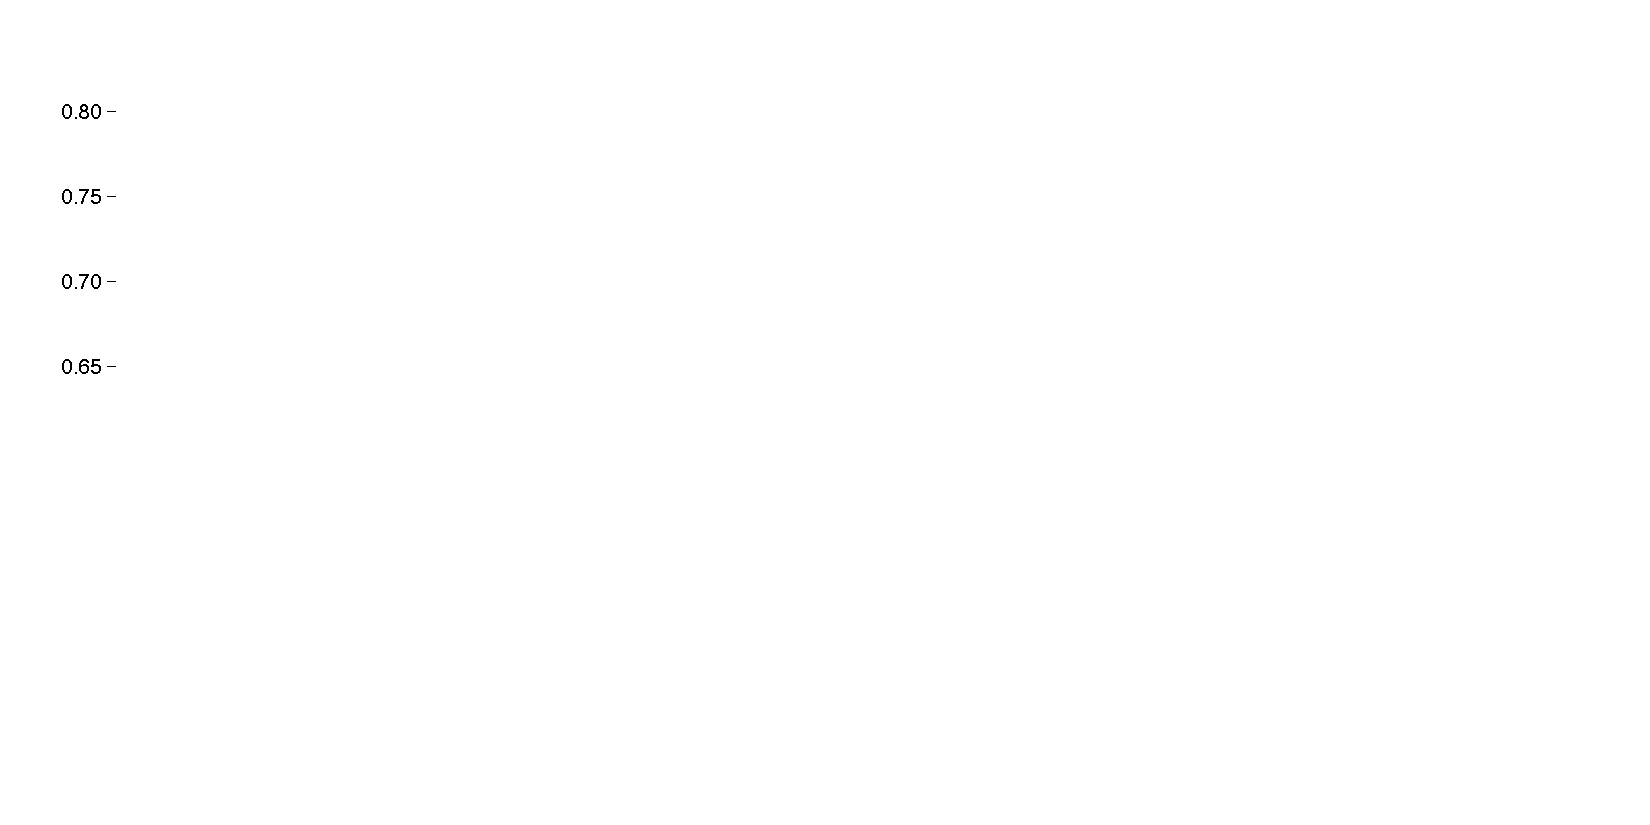
\includegraphics[scale=\graphscale]{reading_tea_leaves/tasks/mp_y}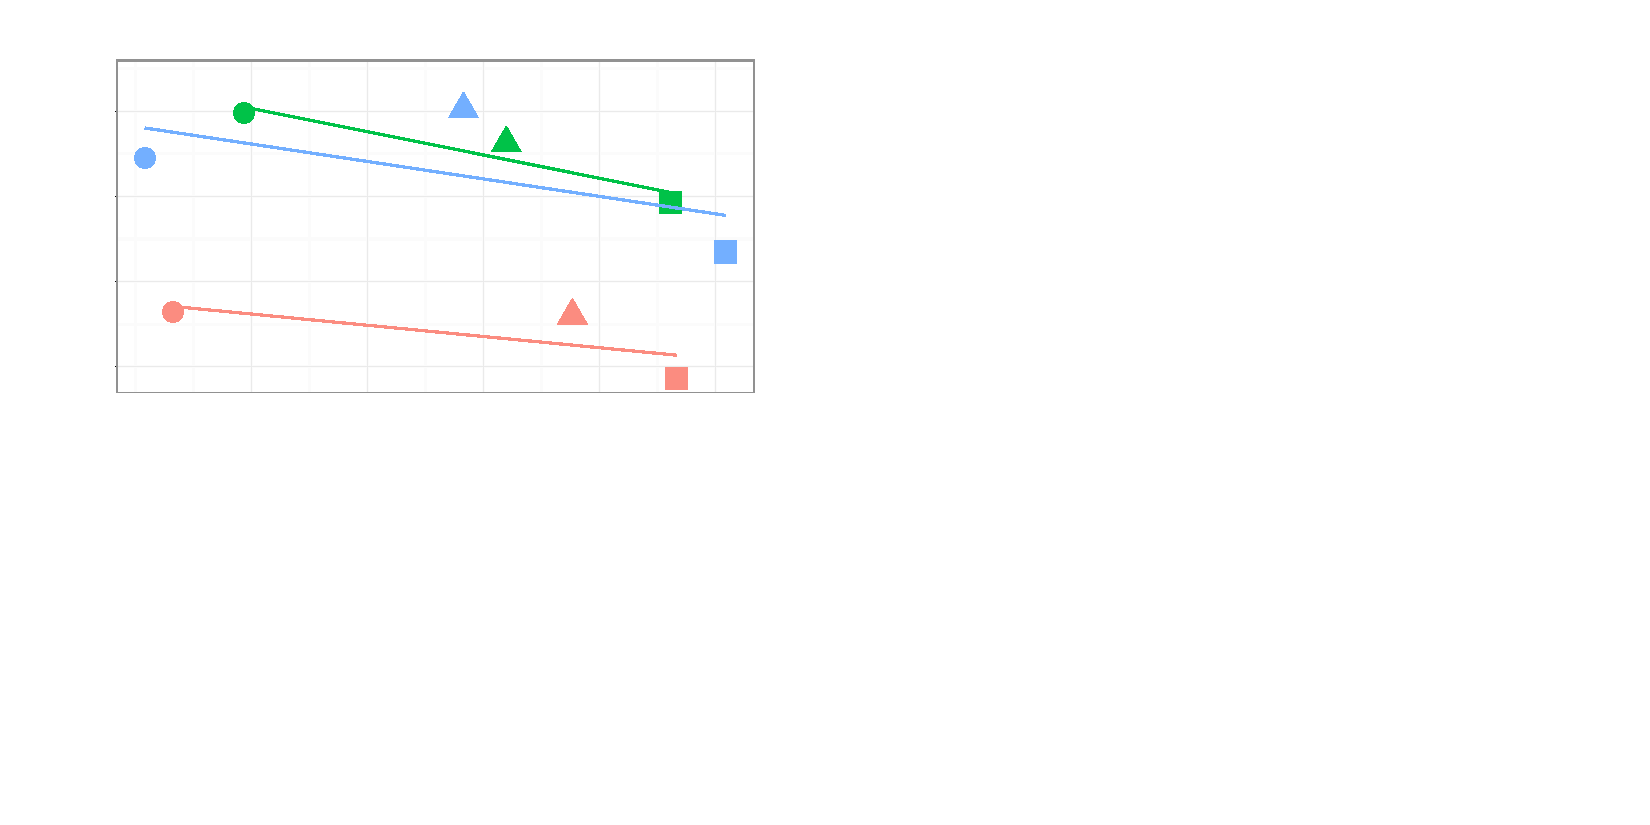
\includegraphics[scale=\graphscale]{reading_tea_leaves/tasks/nyt_mp}\\}
  \only<1>{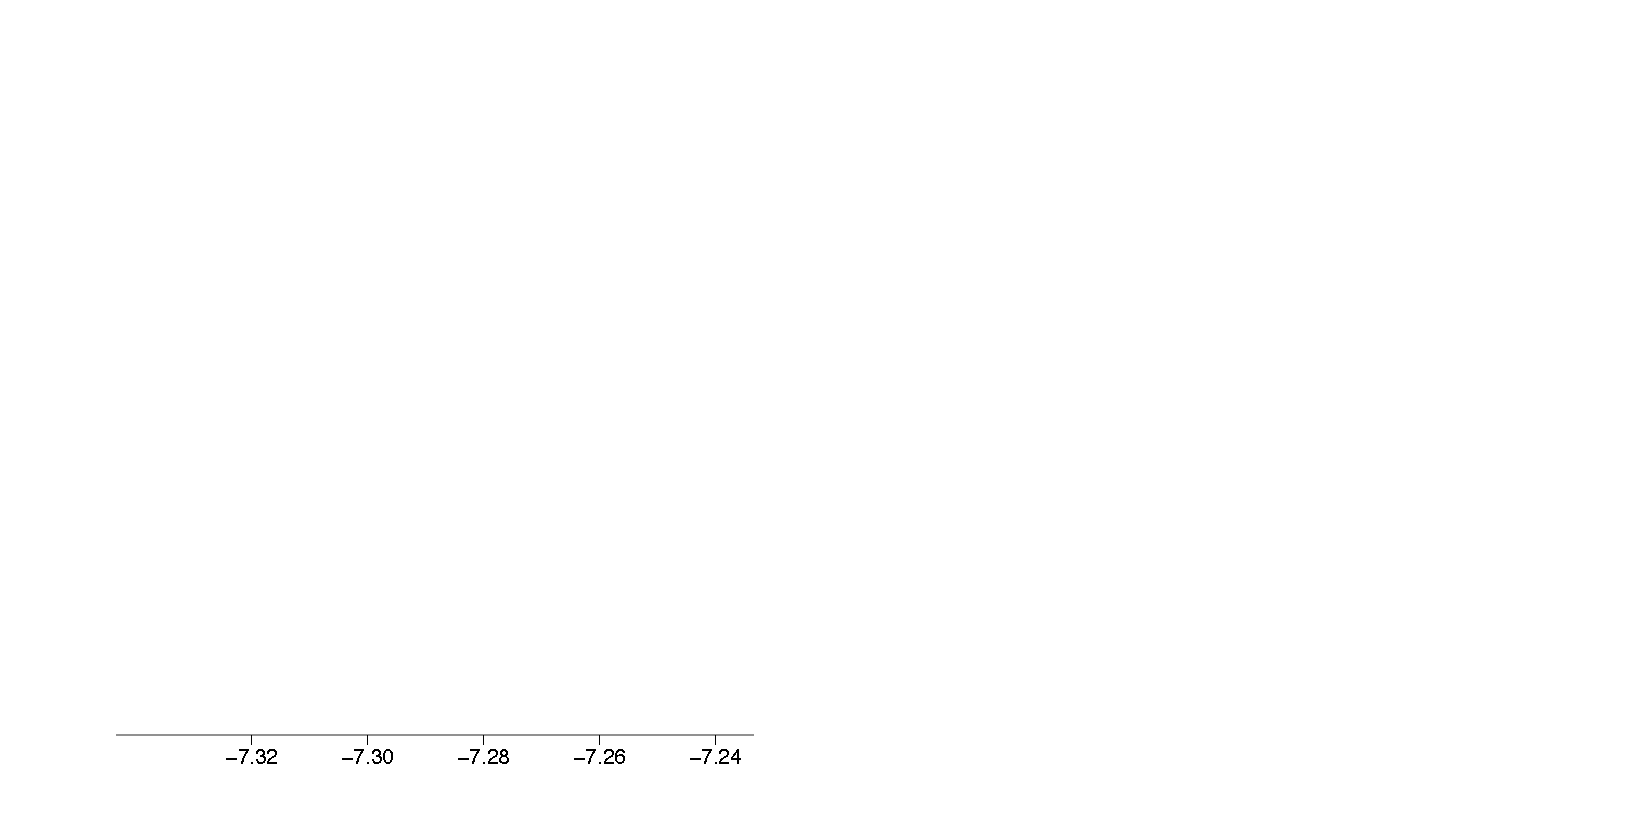
\includegraphics[scale=\graphscale]{reading_tea_leaves/tasks/nyt_x}}

\end{flushright}
\column{.15\linewidth}
  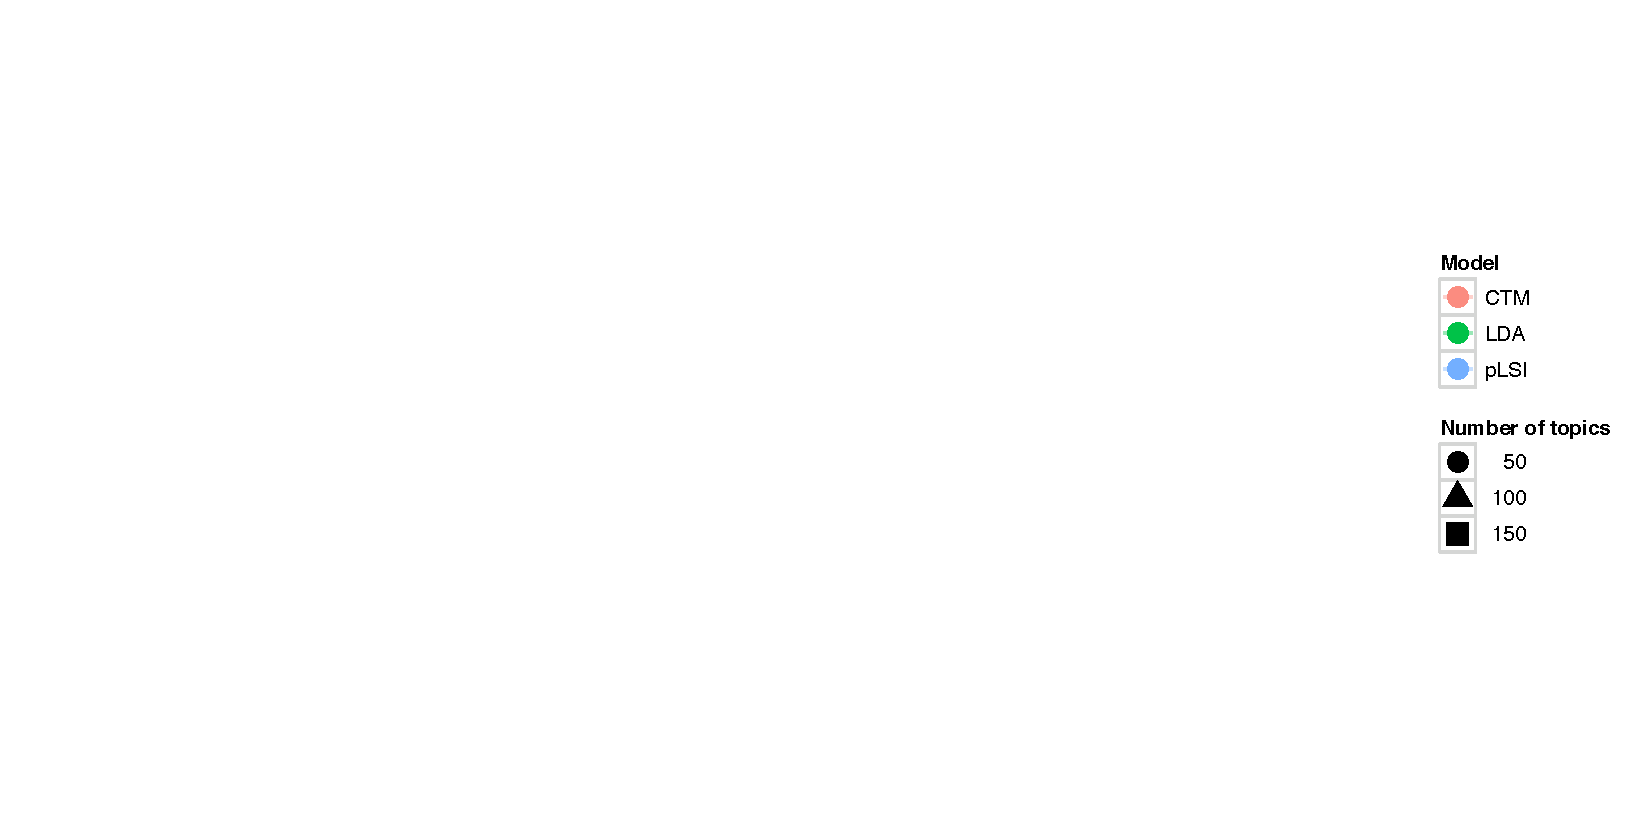
\includegraphics[scale=\graphscale]{reading_tea_leaves/tasks/legend}
\end{columns}
\vspace{-0.75cm}
\begin{center}
  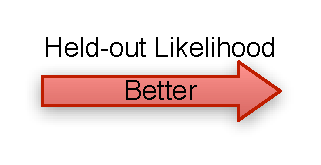
\includegraphics[scale=\graphscale]{reading_tea_leaves/tasks/held-out} \\
\only<1> {within a model, higher likelihood $\not =$ higher interpretability}
\end{center}
}


\begin{frame}{Since then \dots}

  \begin{itemize}
    \item A way to get at an evaluation that matches {\bf what we care about}
    \item A necessary step to improving topic models for navigating large datasets~\cite{talley-11}
    \item Others have discovered automatic methods that uncover the same properties~\cite{newman-10,mimno-11}
    \item And extended the technique to structured topics and phrases~\cite{lindsey-12,weninger-12}
  \end{itemize}

\end{frame}
